\documentclass[12pt]{article}
\usepackage[left=0cm, right=0cm, top=2cm]{geometry}
\usepackage{amsfonts,amssymb,amsmath,graphicx,physics,array,mathrsfs,cancel,textcomp}
\begin{document}

\title{Likelihood Expression}
\author{Daniel Sullivan}
\date{\today}
\maketitle


$$P(G|\lambda,\mu,\theta)=\int_{S}^{}P(G|S,\theta)P(S|\lambda,\mu)$$
$$\int_{0}^{\infty}...\int_{0}^{\infty}\prod_{pop=1}^{n_{leaves}-1}\left[\prod_{j=n_{pop}+1}^{m_k+m_l}\left[\frac{2}{\theta}\exp^{\frac{-j(j-1)}{\theta}}t_j\right]*\exp^{\frac{(m_k+m_l)(m_k+m_l-1)}{\theta}(\tau_{pop}-(t_{m_k+m_l}+t_{m_k+m_l+1}+...+t_{n_{pop}+1})}\right]\times $$
$$(loucalikelihood)d\tau_1...d\tau_{n_{leaves}-1}$$

$\tau$ is the divergence time of the species

need to somehow  marginalize (sum) over all possible scenarios of lineages coming in and going out of species branches. 

The topology of the species tree is still encoded in the way that gene lineages go in and out of species branches because we need to know the daughter-parent realtionships.  

$n_{leaves}-1$ internal nodes/species divergence times

1 representative from each species at each leaf for now so that the number of lineages entering a branch can only be as large as the number of leaves that are descended from that branch. 

$m_k,m_l$ are $n_{pop}$ for the daughter branches, they are the number of lineages leaving those branches.

number of lineages entering is at minimum 2. 

change of variable to difference between species branch lengths? instead of just species divergence times, look at differences in species divergence times. 

$$\sum_{daught1out=1}^{daught1in}\sum_{daught2out=1}^{daught2in}\sum_{parentout=1}^{daught2out+daught1out}$$
The variables with the suffix "out" descibe the number of lineages exiting the branch with the name corresponding to the prefix, and those with the suffix "in" describe the number of lineages entering a branch with the name corresponding to the prefix.
\newline
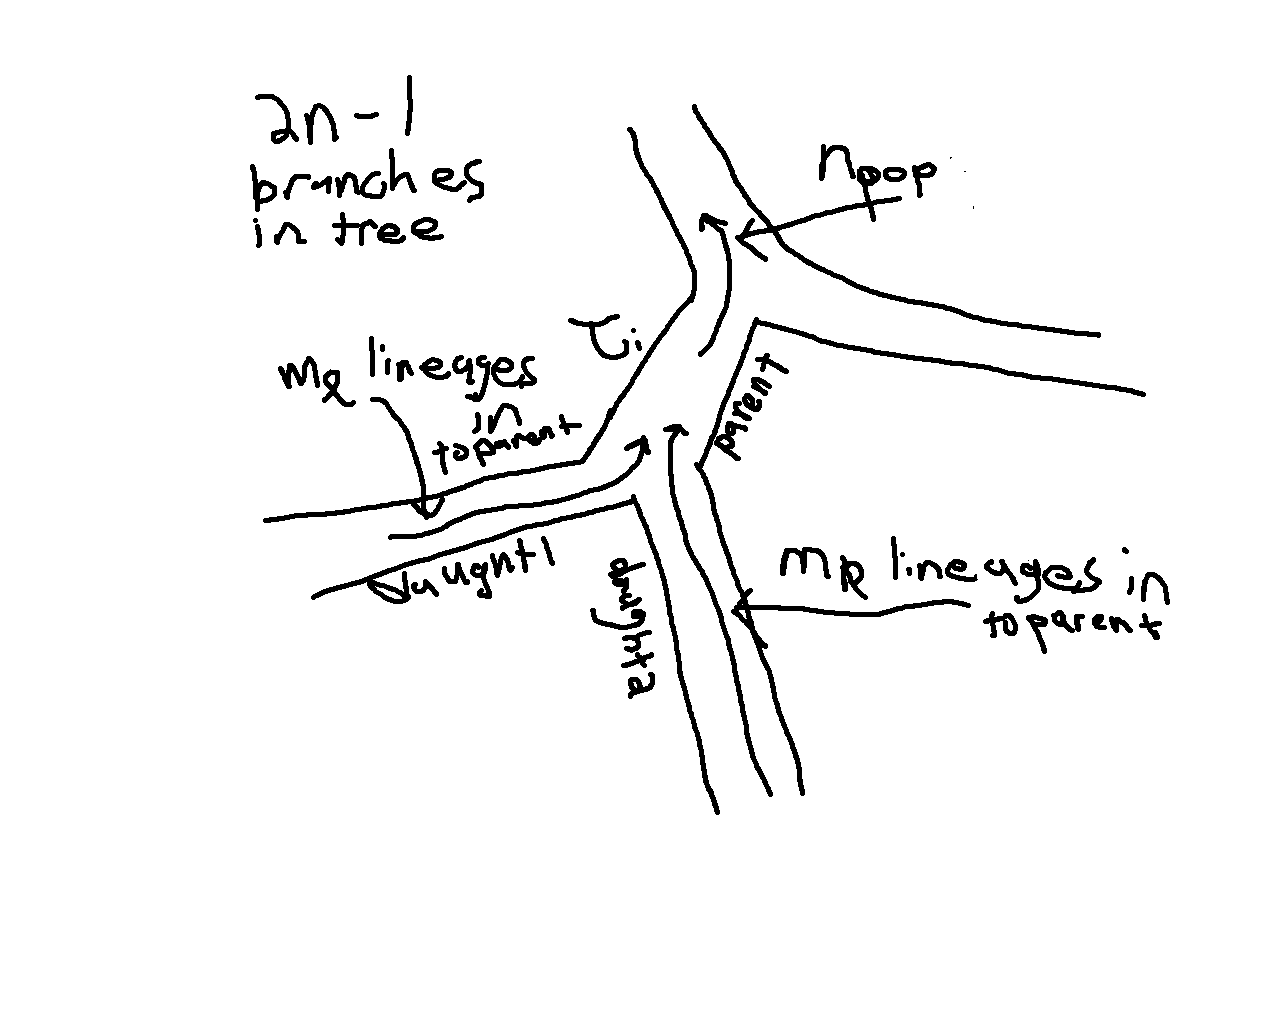
\includegraphics[scale=0.4]{coalescentdrawings.png}
\end{document}